To achieve our goal of a modular analysis of modification for feature model evolution plans, we first need a representation that supports local lookup and modification. Using the representation we defined in the paper~\cite{art:consistency-preserving-evolution-planning} , with an initial model followed by a list of operations associated with time points, would not serve us, as the operations have to be applied in order to retrieve the state (current feature model) at any point in time. In this chapter we present the definitions required for our representation, the operations for editing plans, and their scopes.

\section{Interval-Based Feature Model}
\label{sec:interval-based-feature-model}

\begin{definition}[Interval-based feature model]
  An \emph{interval-based feature model} is defined as a triple $(\names, \features, \groups)$ where \names{} is a \emph{map} from names to \emph{interval maps} with feature ID values, \features{} is a map from feature IDs to \emph{feature entries}, and \groups{} is a map from group IDs to \emph{group entries}. 
  \label{def:interval-based-feature-model}
\end{definition}

The reason for this choice is mainly modularity. As previously mentioned, the goal of this thesis is to minimize the scope of the plan to check for paradoxes, as a change rarely affects more than a small part of the plan. It would then be a mistake to represent a plan as a sequence of trees associated with time points, or an initial model followed by a sequence of operations as described in \citetitle{art:consistency-preserving-evolution-planning} \parencite{art:consistency-preserving-evolution-planning}. To add a new feature to the plan, both representations would require us to look through the entire plan to check that the feature ID is fresh.

To add or rename a feature, a soundness checker must verify that no other feature is using the name during the affected part of the plan. We therefore include the \names{} map in the representation for efficient verification of aforementioned issue. A feature or group ID may not already be in use when we add it, so the \features{} and \groups{} maps support efficient lookup for IDs. The rest of this section gives more detailed explanations of interval-based feature models.

\section{Maps}
\label{sec:maps}

\begin{definition}[Map]
  A \emph{map} is a set of entries on the form $\mapping{k}{v}$, where each key $k$ uniquely defines a value $v$. 
  \label{def:map}
\end{definition}

Following is the syntax for looking up a value at the key $k$ in map \map{map}:
\[
  \lookup{\map{map}}{k}
\]

This query would give us $v$ if $\mapping{k}{v} \in \map{map}$. If we wish to assign a value $v'$ to key $k$, this is the syntax:
\[
\lookup{\map{map}}{k} \assign v'
\]
The semantics of assignment is given by the following:
\begin{align*}
  \lookup{\left(\map{map} \cup \set{\mapping{k}{v}}\right)}{k} \assign v' &= \map{map} \cup \set{\mapping{k}{v'}} &&\\
  \lookup{\map{map}}{k} \assign v' &= \map{map} \cup \set{\mapping{k}{v'}} && \text{if $k$ is not a key in \map{map}}
\end{align*}
Note that we do not mutate maps, but rather obtain a new map when assigning a value to a key. 

For maps with set values, we define an additional operator $\addassign$. If $\lookup{\map{map}}{k} = S$ then 
\[\lookup{\map{map}}{k} \addassign v = \lookup{\map{map}}{k} \assign S \cup \{v\}\]
To remove a mapping with key $k$, we use $\map{map} \setminus k$. For maps with set values, we additionally define $\removevalue{v}$, where $v$ is some value. Let $\map{map}$ be a map with set values containing the mapping $\mapping{k}{\{v\} \cup S}$. Then $\removevalue{v}$ is defined as follows:

\[
  \map{map} \removevalue{v} k =
  \begin{cases}
    \map{map} \remove k & \text{if } S = \emptyset\\
    \lookup{\map{map}}{k} \assign S & \text{if } |S| > 0
  \end{cases}
\]
That is, if removing $v$ leaves only the empty set at $\lookup{\map{map}}{k}$, we remove the mapping. Otherwise, we only remove $v$ from the set of values associated with $k$. 

\section{Intervals}
\label{sec:intervals}
To define the map values used in interval-based feature models, we must first define an \emph{interval}.
\begin{definition}[Interval]
  An interval is a set of time points between a lower and an upper bound. We denote the interval using the familiar mathematical notation $\interval{t_\text{start}}{t_\text{end}}$, where $t_\text{start}$ is the lower bound, and $t_\text{end}$ is the upper bound. These intervals are left-closed and right-open, meaning that $t_\text{start}$ is contained in the interval, and all time points until but not including $t_\text{end}$.
  \label{def:interval}
\end{definition}

To allow us to use intervals that have no end, we define the time point $\forever$, such that $\interval{1}{\forever}$ is an interval that starts at $1$ and never ends. For all time points $t_n$, we have that $t_n \leq \forever$. 

We say that an interval $\interval{t_\text{start}}{t_\text{end}}$ \emph{contains} the time point $t_k$ if $t_\text{start} \leq t_k < t_\text{end}$. Two intervals $\interval{t_n}{t_m}$ and $\interval{t_i}{t_j}$ \emph{overlap} if there exists a time point $t_k$ with $t_n \leq t_k < t_m$ and $t_i \leq t_k < t_j$, i.e. a time point contained by both intervals.

For intervals $\interval{t_{start}}{t_{end}}$ with unknown bounds, we may restrict the bounds to $t_l$ and $t_r$ by writing $\clamp{\interval{t_{start}}{t_{end}}}{t_l}{t_r}$. We then get the interval $\interval{\textbf{max}(t_{start}, t_l)}{\textbf{min}(t_{end}, t_r)}$.

\section{Interval Maps}
\label{sec:interval-maps}
\begin{definition}[Interval map]
An \emph{interval map} is a map where the key is an interval (Definition~\vref{def:interval}). 
  \label{def:interval-map}
\end{definition}

To look up values, one can either give an interval or a time point as key. Both will return sets of values. For instance, if an interval map \map{IM} contains the mapping $\intervalmapping{t_1}{t_5}{v}$, all of the queries in Figure~\vref{ex:interval-map} will return $\{v\}$ (assuming that $t_1 < t_2 < \ldots < t_5$):

\begin{figure}[h]
  \begin{align*}
    & \lookup{\map{IM}}{t_1} \\
    & \lookup{\map{IM}}{t_3} \\
    & \lookup{\map{IM}}{\interval{t_1}{t_5}} \\
    & \lookup{\map{IM}}{\interval{t_2}{t_4}}
  \end{align*}
  \caption{Interval map example}
  \label{ex:interval-map}
\end{figure}

$\containing{\map{IM}}{t_n}$ returns the set of keys containing time point $t_n$. For interval maps with non-overlapping keys, the resulting set will contain at most one element. For interval maps with set values, we define an additional function $\containingvalue{\map{IM}}{t_n}{v}$ where $v$ is some value, returning the set of the keys containing $t_n$ and associated with a set containing $v$. 

We furthermore define function $\overlapping{\map{IM}}{t_n}{t_m}$ which returns all the interval keys in the map $\map{IM}$ overlapping the interval $\interval{t_n}{t_m}$. 

Assigning a value $v$ to an empty interval in a map $\map{IM}$ returns the same map, i.e. it is a no-op. Formally,
\[
  \lookup{\map{IM}}{\interval{t_n}{t_n}} \assign v = \map{IM}
\]
Likewise, the empty mapping $\intervalmapping{t_n}{t_n}{v}$ is ignored, such that
\[
  \map{IM} \cup \set{\intervalmapping{t_n}{t_n}{v}} = \map{IM}
\]

\section{Interval Sets}
\label{sec:interval-sets}

\begin{definition}[Interval set]
  An \emph{interval set} is a set of intervals (Definition~\vref{def:interval}). 
\end{definition}

Given an interval set $\map{IS}$, $\interval{t_n}{t_m} \in \map{IS}$ if $\interval{t_n}{t_m}$ is a member of the set, which is the expected semantics of $\in$. We define a similar predicate $\inn$ such that $\interval{t_n}{t_m} \inn \map{IS}$ iff there exists some interval $\interval{t_i}{t_j} \in \map{IS}$ with $t_i \leq t_n \leq t_m \leq t_j$, i.e. an interval in $\map{IS}$ which contains $\interval{t_n}{t_m}$. We further define the predicate $\innr$ such that $\interval{t_n}{t_m} \innr \map{IS}$ iff there exists some interval $\interval{t_i}{t_j} \in \map{IS}$ with $\interval{t_n}{t_m}$ overlapping $\interval{t_i}{t_j}$. 

Notice that if $\interval{t_n}{t_m} \in \map{IS}$ then also $\interval{t_n}{t_m} \inn \map{IS}$, and $\interval{t_n}{t_m} \innr \map{IS}$. Thus $\in$ is the strictest, and $\innr$ the most general.

We also define $\inn$ for time points $t_n$, so that $t_n \inn \map{IS}$ if some interval $\interval{t_i}{t_j} \in \map{IS}$ with $t_i \leq t_n < t_j$. 

$\containing{\map{IS}}{t_n}$ returns the subset of $\map{IS}$ containing $t_n$.

\section{Map Entries}
\label{sec:map-entries}
Each feature, group, and name should be available at the top level, so as to make sure names and IDs are unique at some time. However, all their parts are variable. A name may be used by several features at different times. A group may move, change its type, or be removed, and a feature can do all of the former as well as change its name. Thus all of this information must be captured in the map entries; if we look up a name, we should find all its usages, and if we look up a feature or a group, \emph{all} the information about its variations must be available. We therefore design the map entries with this in mind.

\subsection{Mapping Names}
\label{sub:mapping-names}

The \names{} map has entries of the form $\mapping{\name{}}{\textit{interval map}}$. Assuming $\mapping{\var{name}}{\map{Im}} \in \names$, the interval map \map{Im} contains mappings on the form $\intervalmapping{t_\text{start}}{t_\text{end}}{\var{featureID}}$, where \var{featureID} is the ID of some feature in the interval-based feature model. This should be interpreted as ``\emph{The name \emph{\var{name}} belongs to the feature with ID \emph{\var{featureID}} from $t_{\emph{\text{start}}}$ to $t_{\emph{\text{end}}}$}". Looking up a name which does not exist will return an empty map $\emptyset$. 

This map is mainly used when adding features or changing names. The new name and the scope of the change is then looked up in the \names{} map to verify that no other feature shares the name.

\subsection{Mapping Features}
\label{sub:mapping-features}

The \features{} map has entries of the form $\mapping{\var{featureID}}{\textit{feature entry}}$. Since several pieces of information are crucial to the analysis of a feature, it is not enough to have a simple mapping as we have for names.
A feature has a name, a type, a parent group, and zero or more child groups. Furthermore, a feature may be removed and re-added during the course of the plan, so we also need information about when the feature exists.
This information is collected into a 5-tuple $\feature$, where $F_e$ is an interval set denoting when the feature exists, $F_n$ is an interval map with name values, $F_t$ is an interval map with the feature's variation types, $F_p$ is an interval map with group ID values, and $F_c$ is an interval map where the values are sets containing group IDs, the interval keys possibly overlapping.

Looking up a feature which does not exist returns an empty feature $(\emptyset \comma \emptyset \comma \emptyset \comma \emptyset \comma \emptyset)$. This lets us treat an unsuccessful lookup the same way as a successful one.

The root ID is constant for a interval-based feature model. We assume that it has been computed and is stored in the variable $\var{rootID}$. 

The reasoning behind the choice of interval sets and maps here is in large part the temporal scope; for instance, when a feature is removed, we can easily look up the temporal scope in the $F_c$ map (child groups) to verify that removing the feature leaves no group without a parent.

\subsection{Mapping Groups}
\label{sub:mapping-groups}

The \groups{} map has entries of the form $\mapping{\var{groupID}}{\textit{group entry}}$. A group has a type, a parent feature, and zero or more child features. These can all be defined in terms of intervals and collected into a 4-tuple similarly to the feature entries $\group$, where $G_e$ is an interval set denoting when the group exists, $G_t$ is an interval map with the group's types, $G_p$ is an interval map with parent feature IDs, and $G_c$ is an interval map with child feature ID set values, the interval keys possibly overlapping.

Looking up a group which does not exist in the map returns an empty group $(\emptyset \comma \emptyset \comma \emptyset \comma \emptyset)$. 

\section{How to Use the Interval-Based Feature Model}
\label{sec:how-to-use-the-interval-based-feature-model}
To provide intuition, we give some examples of how to use the interval-based feature model.

If a group with ID $\var{groupID}$ with $\lookup{\groups}{\var{groupID}} = \group{}$ has the type \xortype{} at time $t_2$, then
\[
  \lookup{G_t}{t_2} = \set{\xortype{}}
\]
The result is a set due to the nature of the interval keys; $t_2$ is contained within some interval key in $G_t$. 

Suppose we have a feature with ID $\var{featureID}$ where $\lookup{\features}{\var{featureID}} = \feature{}$. To check whether the feature exists at the time point $t_5$, we look up the time point in the feature's existence set $F_e$. Recall that $F_e$ is an interval set. Then
\[
  t_5 \inn F_e
\]
means that $t_5$ is contained within some interval in $F_e$, so the feature does exist at time $t_5$. We use the operator $\inn$ because the elements in $F_e$ are intervals, and we wish to know whether $t_5$ is contained within one of those intervals. To get the feature's parent group ID at time $t_5$, we look up the time point in the feature's parent map $F_p$:
\[
  \lookup{F_p}{t_5} = \set{\var{parentGroupID}}
\]
This is exactly the same as how we previously used $\lookup{G_t}{t_2}$. The resulting set $\set{\var{parentGroupID}}$ means that the only parent group the feature has at time $t_5$ is $\var{parentGroupID}$. Since the model is assumed to be sound, it makes sense that a feature which exists has exactly one parent group. If the feature did not exist, it would not have a parent group. The result would then be
\[
  \lookup{F_p}{t_5} = \emptyset
\]
Although a feature always has exactly one parent group if it exists, it may have several child groups. Recall that the child group map $F_c$ has set values, meaning that the values are sets of group IDs. Furthermore, the keys may overlap, since a feature may have 3 groups from $t_3$ to $t_6$, but 1 in the interval $\interval{t_4}{t_6}$. Thus, to obtain the set of child groups at time $t_5$, we must take the union of the result after looking up $t_5$ in the child group map $F_c$.
\[
  \bigcup{\lookup{F_c}{t_5}} = \set{\var{childGroup1}, \var{childGroup2}, \var{childGroup3}, \var{childGroup4}}
\]
If we did not take the union, we would get something like
\[
  \lookup{F_c}{t_5} = \set{\set{\var{childGroup1}, \var{childGroup2}, \var{childGroup3},} \set{\var{childGroup4}}}
\]
This is why, later in the thesis, we see expressions like
\[
  \var{groupID} \in \bigcup{\lookup{F_c}{t_n}}
\]
This expression means that the group with ID $\var{groupID}$ is a child group of our feature at time $t_n$.

Furthermore, we sometimes wish to locate the time when something ends; for instance, when a feature stops existing. If we want to find out when our feature is next removed after $t_5$, we can look it up in the existence set:
\[
  \containing{F_e}{t_5} = \set{\interval{t_2}{\forever}}
\]
The result set means that the feature is added at $t_2$, and is never removed. The syntax looks exactly the same for interval maps. If we want to know when the feature is next moved (after $t_5$), we use the same operator with the parent group map:
\[
  \containing{F_p}{t_5} = \set{\interval{t_3}{t_6}}
\]
The feature was moved to its current parent group at $t_3$, and will be moved next at $t_6$.

We often want to know what is true for an \emph{interval}, not just a time point. In particular, we may want to check that the feature does not exist during some interval, for instance $\interval{t_0}{t_2}$. We then use the negated overlapping member operator $\notinnr$:
\[
  \interval{t_0}{t_2} \notinnr F_e
\]
This predicate is true if no intervals in the set $F_e$ overlaps $\interval{t_0}{t_2}$. If we had that $\interval{t_1}{t_3} \in F_e$, the above predicate would be false, since both intervals contain the time point $t_1$.

\subsection{Example Evolution Plan}
A small example of an interval-based feature model can be found in Figure~\vref{ex:washing-machine}. It contains three features and one group, and describes an interval-based feature model for a washing machine. The washing machine always has a washer, and a dryer is added at $t_5$. 

\begin{figure}
  \begin{align*}
    ( \{ \; & \mapping{\text{Washing Machine}}{\intervalmapping{t_0}{\forever}{0}} \\
       ,\; & \mapping{\text{Washer}}{\intervalmapping{t_0}{\forever}{1}} \\
       ,\; & \mapping{\text{Dryer}}{\intervalmapping{t_5}{\forever}{2}}\; \} \\
       \\
       ,\{\; & \mapping{0}{(\{ \interval{t_0}{\forever}\} ,\, \\
             & \{\intervalmapping{t_0}{\forever}{\text{Washing Machine}}\} ,\, \\
             & \{\intervalmapping{t_0}{\forever}{\mandatory{}}\} ,\, \\
             &  \emptyset ,\, \\ 
             & \{\intervalmapping{t_0}{\forever}{10}\} ) } \\
             ,\, & \mapping{1}{(\{\interval{t_0}{\forever}\} ,\, \\
             & \{\intervalmapping{t_0}{\forever}{\text{Washer}}\} ,\, \\
             & \{\intervalmapping{t_0}{\forever}{\mandatory{}}\} ,\, \\
             &  \{\intervalmapping{t_0}{\forever}{10}\} ,\, \\ 
             & \emptyset)} \\
             ,\, & \mapping{2}{(\{\interval{t_5}{\forever}\} ,\, \\
             & \{\intervalmapping{t_5}{\forever}{\text{Dryer}}\} ,\, \\
             & \{\intervalmapping{t_5}{\forever}{\optional{}}\} ,\, \\
             &  \{\intervalmapping{t_5}{\forever}{10}\} ,\, \\ 
             & \emptyset)} \}\\
             \\
               ,\; \{ \; & [ 10 \mapsto (\{\interval{t_0}{\forever}\} ,\, \\
                         & \{\intervalmapping{t_0}{\forever}{\andtype{}}\} ,\, \\
                         & \{\intervalmapping{t_0}{\forever}{0}\} ,\, \\
                         & \{\intervalmapping{t_0}{\forever}{1},\, \intervalmapping{t_5}{\forever}{2}\} ) ]\\
    \}&)\\
  \end{align*}
  \caption{Small interval-based feature model}
  \label{ex:washing-machine}
\end{figure}

The same plan can be viewed in Figure~\vref{ex:washing-machine-visual}. It is clear from this example that the representation is better suited for manipulating the structure than reading it. 

\begin{figure}
  \centering
  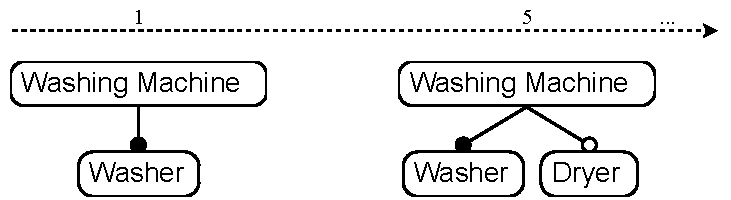
\includegraphics{WashingMachine}
  \caption{Washing machine visualisation}
  \label{ex:washing-machine-visual}
\end{figure}

\section{Operations}
\label{sec:operations}

We define \emph{operations} to alter the interval-based feature model. The choice of operations is in large part based on the edit operations defined in our paper~\cite{art:consistency-preserving-evolution-planning}. We adapt them by adding a temporal dimension, letting us specify both \emph{where} an operation should be applied in the feature model, and \emph{when}, i.e. at which stage of the plan. We give a brief summary of the requirements a plan must fulfil for the operations to be applied.

\begin{itemize}
  \item \textbf{addFeature(featureID, parentGroupID, name, featureType)} from $t_n$ to $t_m$\\
    Adds feature with ID \var{featureID}, name \var{name}, and feature variation type \var{featureType} to the group with ID \var{parentGroupID} in the interval $\interval{t_n}{t_m}$. No feature with ID \var{featureID} must exist during the interval, and the name cannot belong to any other feature in the model during the interval. The parent group must exists during the interval, and the types of the feature and the parent group must be compatible. If the feature has type \mandatory{}, then the parent group must have type \andtype{}. We choose to let this operation affect an interval so as to enable the adding of features to groups that are planned to be removed, and to add flexibility.
  \item \textbf{addGroup(groupID, parentFeatureID, groupType)} from $t_n$ to $t_m$\\
    Adds group with ID \var{groupID} and type \var{groupType} to the feature with ID \var{parentFeatureID} during the interval $\interval{t_n}{t_m}$. The group ID not be in use during the interval, and the parent feature must exist during the entire interval. 
  \item \textbf{removeFeature(featureID)} at time $t_n$\\
    Removes the feature with ID \var{featureID} from the feature model at $t_n$. If the plan contains a removal of the feature and a subsequent reintroduction, removing the feature at an earlier stage does not affect the reintroduction. The feature must exist at $t_n$ in the original plan for the modification to be valid. The feature must not have any child groups that are left orphaned after removal. 
  \item \textbf{removeGroup(groupID)} at time $t_n$\\
    This operation is very similar to \textbf{removeFeature}. Removes the group with ID \var{groupID} from the feature model at $t_n$, not affecting potential later reintroductions. The group must exist at $t_n$ in the original plan, and the group must not have any child features that are left orphaned after removal. 
  \item \textbf{moveFeature(featureID, targetGroupID)} at $t_n$\\
    Moves the feature with ID \var{featureID} to the group with ID $\var{targetGroupID}$ at $t_n$. The operation does not affect future moves planned for the feature. The feature's subtree is moved along with the feature. The move cannot be done if it introduces a cycle; that is, if the target group is in the feature's subtree at some point in the plan. Furthermore, the target group's type must be compatible with the feature's type, i.e. if the feature is \mandatory{} and the group is \optional{}, the move cannot be done.
  \item \textbf{moveGroup(groupID, targetFeatureID)} \\
    This operation is very similar to \textbf{moveFeature}. It moves the group with ID \var{groupID} to the feature with ID $\var{targetFeatureID}$ at $t_n$. The operation does not affect future moves planned for the group. The group's subtree is moved along with the group. If the move causes a cycle, then the modification should not be applied.
  \item \textbf{changeFeatureVariationType(featureID, newType)} \\
    Changes the feature variation type of the feature with ID \var{featureID} to \var{newType}. The change does not affect planned type changes to the feature. If the new type is \mandatory{}, the parent group type must be \andtype{}, or else the operation cannot be applied.
  \item \textbf{changeGroupVariationType(groupID, newType)}\\
    Changes the group variation type of the group with ID \var{groupID} to \var{newType}. If the new type is \ortype{} or \xortype{}, and a child feature has type \optional{}, then the operation cannot be applied. 
  \item \textbf{changeFeatureName(featureID, name)}\\
    Changes the name of the feature with ID \var{featureID} to \var{name}. It does not affect future renaming operations to the feature. No other feature may have the same name.
\end{itemize}

The operations given above cover most o changes that are likely to be desired for a feature model evolution plan. However, they do not allow for extending or delaying operations, e.g. adding a feature at time 1 instead of at time 3, or changing a group's type to \optional{} at time 5 instead of at time 2.
